To address the new requirement, the architecture will need to be transformed in such a way as to harden the design against the vulnerability.
BriefCASE provides a library of model transformations for addressing common cyber vulnerabilities.  Currently, the following transformations are supported:

% add a brief description for these?
\begin{itemize}
	\item Attestation
	\item Filter
	\item Monitor
	\item Virtualization
	\item Proxy
	\item Switch
	\item seL4
\end{itemize}  

The transformations are automated by the tool, resulting in a hardened model that is correct-by-construction.  
For example, ensuring a component only receives well-formed messages can be accomplished by the insertion of a high-assurance filter.  The BriefCASE Filter transform wizard (Figure~\ref{fig:filter-wiz}) enables the configuration of filter component properties, including the filter behavioral specification, which is represented in the AGREE language.

\begin{figure}[h]
	\centering
	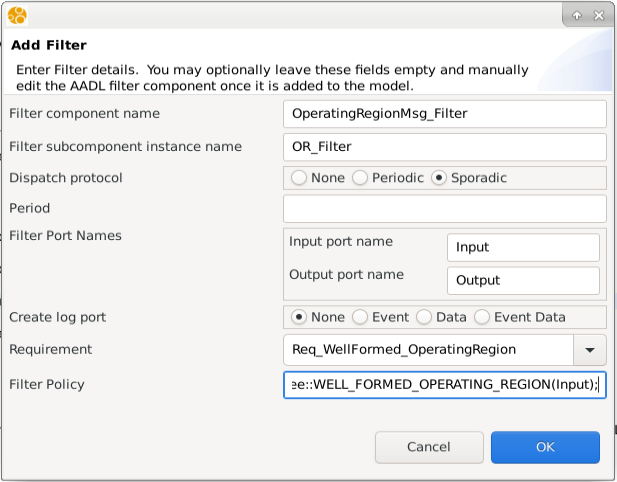
\includegraphics[width=0.7\columnwidth]{figs/filter-wiz.png}
	\caption{Filter transform wizard.} 
	\label{fig:filter-wiz} 
\end{figure}

BriefCASE inserts a new filter component into the model, sets the component properties, and establishes the appropriate connections to source and destination components. The filter specification is inserted into an AGREE annex, enabling both formal analysis of the model as well as providing the behavioral specification for a provably correct synthesis of the component implementation via the SPLAT plugin.

The transformation also updates the Resolute goal with new evidential statements pointing to evidence that the model has indeed been hardened against the vulnerability and the requirement has been satisfied. 
%(as shown in Figure~\ref{fig:resolute-add-filter}).
%For example, the \texttt{add\_filter} strategy is included in a library of built-in Resolute transform rules and provides Resolute with the logical instructions for evaluating if the top-level goal has been satisfied.
%The \texttt{add\_filter} definition (shown in Figure~\ref{fig:resolute-add-filter}) includes the following sub-goals: 
%\begin{itemize}
%	\item \texttt{filter\_exists} - the filter component exists in the model
%	\item \texttt{filter\_not\_bypassed} -  there is no alternate pathway in the model that can bypass the filter
%	\item \texttt{filter\_implemented\_correctly} - the filter has been implemented correctly
%\end{itemize}
%
%
%\begin{figure}[h]
%	\centering
%	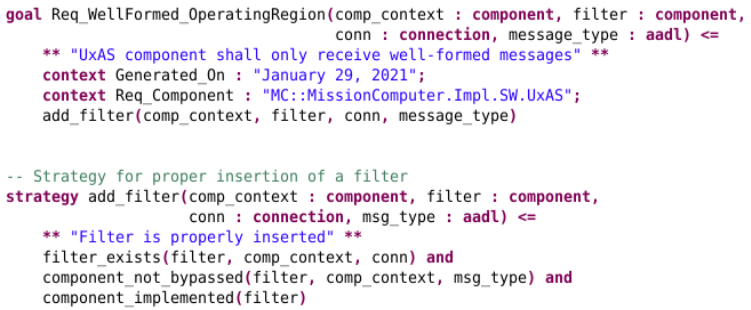
\includegraphics[width=1\columnwidth]{figs/resolute-add-filter.png}
%	\caption{Updated well-formedness claim.} 
%	\label{fig:resolute-add-filter} 
%\end{figure}

%The first two sub-goals are supported by evidence obtained by examining the structure of the model, while the last is determined by examining the output of the synthesis tool.  
%%This approach follows the model-based decomposition pattern based on~\cite{model-based-decomposition}, and is representative of all BriefCASE transform assurance strategies.
%If at a later time during development the model is inadvertently altered in a way that renders the transformation ineffective, Resolute will be unable to substantiate the evidential statements, and therefore produce a failing assurance case.
%
%The third subgoal is satisfied by SPLAT.  SPLAT not only generates the  implementation code for high-assurance components such as filters, monitors, and gates, but it also produces a proof that this code correctly implements its AGREE specification.  
%Resolute uses the existence of the SPLAT proof as evidence that the component was implemented correctly.